\lecture{12}{Mar 5 10:10}{}
\section{Review}
Separation of variables with spherical coordinates will give a special function specifically the spherical harmonics
\[
    Y_v^m (\theta , \phi ) e^{im \phi} P_i^m \cos \theta
\]
FOr the cylindrical coordinates we have the Bessel function
\[
    e^{in \phi } , e^{\pm kz}, \text{ Bessel function} 
\]
\section{Cylindrical Coordinates}
\[
    \Phi (r,\phi ,z) \approx \sum_{m,n} \left[ A_{mn} I_n (k_m r) + B_{mn N_n (l_m r)}  \right] e^{\pm in \phi  \pm kmz}
\]
\begin{eg}
We have a charged wire where \(\phi _0\)  is the flux inside and \(\phi \) on the surface and \(\phi  =0 \) for above the surface.
We know from here that no charge \(\implies B_{mn}  = 0\); symmetry \(\implies n = 0\). Thus we get the equation
\[
    \Phi (r,\phi ,z) = \sum_{m} A_m J_0 (k_m r) e^{-k_m z}
\]
From our boundary conditions we have \(\Phi (a,\phi ,z) = 0\) This type of boundary condition tells the roots and our harmonic is the bessel function. 
Another boundary condition is 
\[
    \Phi (r, \phi , 0) = \phi _0 \to A_m
\]
\begin{figure}[H]
    \centering
    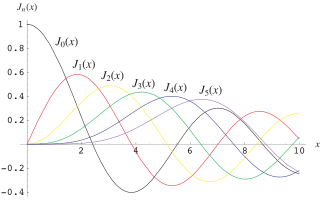
\includegraphics[width=0.4\textwidth]{Figures/BesselJ_800.png}
    \caption{}
    \label{fig:}
\end{figure}
The orthoganality condition we get here is simply
\[
    \int_{0}^{a} J_n (k_m r) J_n (k_L r) \,\mathrm{d}r = \frac{a^{2}}{2} J_{n+1} ^{2}  (k_L a) \delta_{mL} 
\]
\end{eg}

\section{Multipole Expansion}
\begin{figure}[H]
    \centering
    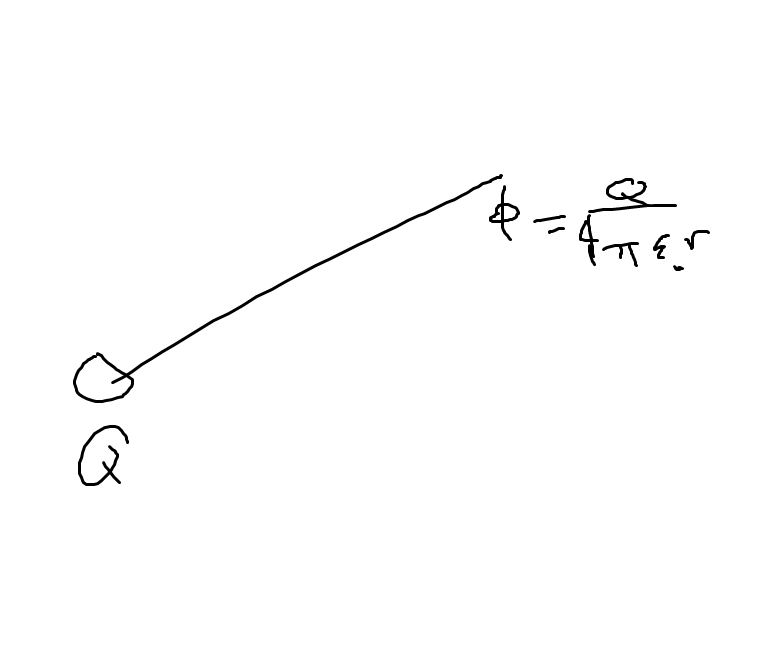
\includegraphics[width=0.4\textwidth]{Figures/05.png}
    \caption{}
    \label{fig:}
\end{figure}figure  
Suppose we had a dipole here, then we will get the form that the potential to be 
\[
    \Phi (\vec{r} ) = \frac{1}{4 \pi \epsilon _0} \left(  \frac{q}{r_+ - \frac{q}{r_-}} \right) 
\]
\[
    \frac{1}{r{\pm}} = \frac{1}{r \sqrt{1 \mp \frac{d}{r}\cos \theta} } \to \frac{1}{r}\left( 1 \pm \frac{d}{2r}\cos \theta \right) 
\]
\[
    \frac{1}{r_+} - \frac{1}{r_-} = \frac{d}{r^{2}} \cos \theta
\]
\[
    \Phi (\vec{r} ) = \frac{1}{4\pi \epsilon _0 } \frac{qd \cos \theta}{r^{2} } \infty \frac{1}{r^{2} }
\]
Thus for monopoles the potential falls off as a function of \(\frac{1}{r}\) and the dipole will hall of as a function of 
\(\frac{1}{r^{2} }\). For quadruples we get that the potential falls as a function as \(\frac{1}{r^{3} }\). If we continue with a cube we will have that the potential fall off
as a function of \(\frac{1}{r^4}\). Thus if we are interested in a far-field approximation we only care about the monopole term, and if 0 then consider the dipole term and continue. 
This is similar to when expanding the potential term as a function of \(\frac{1}{r}\). Thus we can do the following expansion for general charge distributions:
\[
    \Phi (\vec{r} ) = \frac{1}{4\pi \epsilon _0} \int \frac{\rho (\vec{r} ^{\prime} )}{\vert \vec{r} -\vec{r} ^{\prime}  \vert } dV^{\prime} 
\] 
\begin{figure}[H]
    \centering
    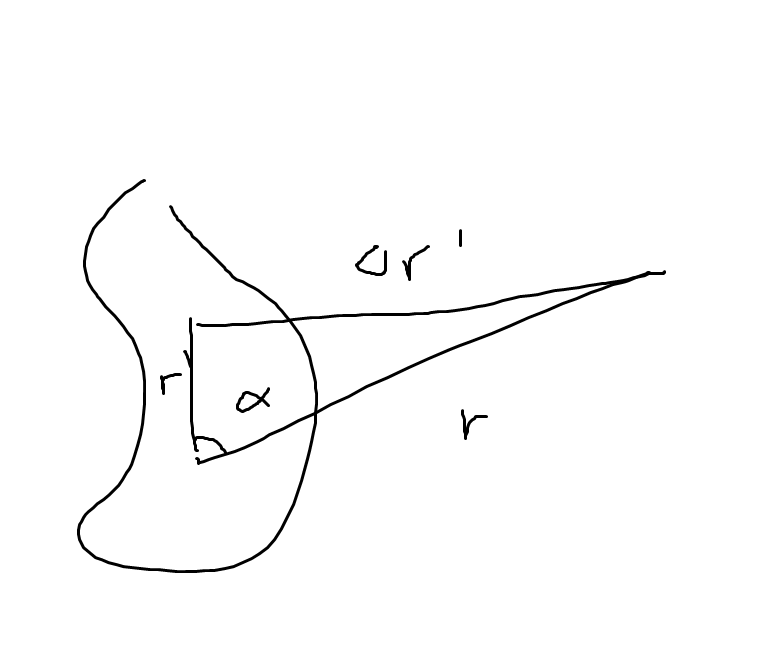
\includegraphics[width=0.4\textwidth]{Figures/06.png}
    \caption{}
    \label{fig:}
\end{figure}
Suppose that we want to calculate the potential \(\vec{r} \) away we get that 
\[
    (\Delta r^{\prime} )^{2} = r^{2} +r^{\prime 2} - 2r r^{\prime}  \cos \alpha = r^{2}  \left[  1+ \left( \frac{r^{\prime} }{r} \right) ^{2} - 2 \frac{r^{\prime} }{r} \cos \alpha \right] 
\]
\[
    \Delta r^{\prime}  = r \sqrt{ 1 + \epsilon }, \epsilon  = \frac{r^{\prime} }{r} \left(  \frac{r^{\prime} }{r} - 2 \cos \alpha \right)  
\]
For \(\frac{r^{\prime} }{r} \to  0, \epsilon  \to  0\)
\[
    \frac{1}{\Delta r^{\prime} } = \frac{1}{r} (1+\epsilon )^{-\frac{1}{2}} = \frac{1}{r} \left( 
        1- \frac{1}{2}\epsilon  + \frac{3}{8}\epsilon ^{2}  - \frac{5}{16} \epsilon ^{3}  + \dots 
     \right)  
\] 
\[
     = \frac{1}{r} \left[  1 + \frac{r^{\prime} }{r} + \left( \frac{r^{\prime} }{r} \right) ^{2} \left(  \frac{3\cos ^{2} \alpha - 1}{2} \right) + \dots  \right] 
\]
which are the Legendre polynomials. 
\begin{figure}[H]
    \centering
    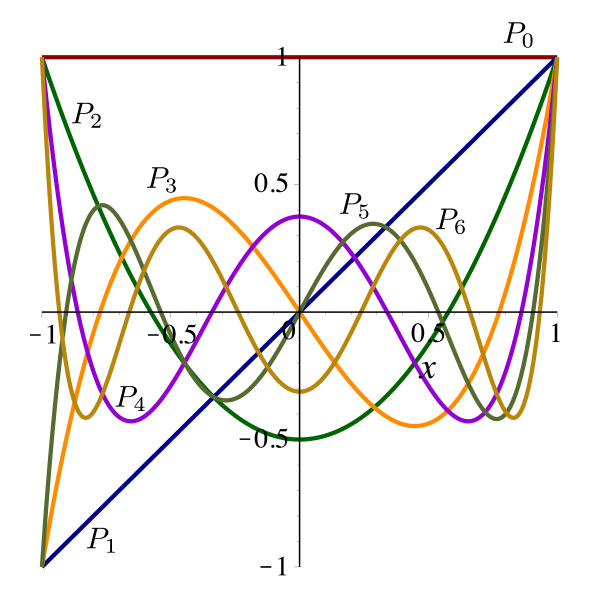
\includegraphics[width=0.5\textwidth]{Figures/07.png}
    \caption{}
    \label{fig:}
\end{figure}
\[
    \frac{1}{\Delta r^{\prime} } = \frac{1}{r} \sum_{n=0}^{\infty} \left(  \frac{r^{\prime} }{r} \right)^n P_n (\cos \alpha) 
\]
\[
    \Phi (\vec{r} ) = \frac{1}{4\pi \epsilon _0} \left[  \frac{1}{r} \int  \rho (\vec{r} ^{\prime} )  dV^{\prime}  + \frac{1}{r^{2}}  \int  r^{\prime}  \cos \alpha \rho (\vec{r ^{\prime} } ) dV^{\prime} +\dots \right] 
\]
We see that the first term gives the monopole and the second term gives the dipole and the third term will give you the quadrupole. Notice that for the physical dipole we are already making some assumptions. However, the formula above for 
\(\Phi (\vec{r} )\) is an exact equation when taking account of higher order terms. Notice the dipole term
\[
    \Phi_{dip} (\vec{r} ) = \frac{1}{4\pi \epsilon _0 } \frac{1}{r^{2} } \int  r^{\prime}  \cos \alpha \rho (r^{\vec{\prime}} ) dV^{\prime} \quad r^{\prime} \cos \alpha = \hat{r} \cdot \vec{r}^{\prime} 
\]
\[
    =\frac{1}{4\pi \epsilon _0} \frac{1}{r^{2} } \hat{r} \cdot \int r^{\vec{\prime}} \rho(\vec{r} ^{\prime} ) dV^{\prime} 
\]
\[
    \Phi_{dip} (\vec{r}) = \frac{1}{4\pi \epsilon _0}\frac{1}{r^{2} } \hat{r}  \cdot \vec{p} 
\]
where the geometry of the charge distribution is  
\[
     \vec{p} = \sum_{i}^{\infty}q_i \vec{r}_i^{\prime} = q \vec{d} 
\]
\begin{remark}
    For the physical dipole, it gives the dipole term only when \(\frac{d}{r} \to 0\). Thus, to construct a mathematical dipole we would need \(d\)to be very small. We see that for the mathematical dipole we have \(\vec{p}  = q \vec{d} \). 
Thus we must have the condition that \(d \to  0\) and \(q \to  \infty \) in order to make \(\vec{p} \) finite.       
\end{remark}
\section{Dependence on Coordinate Origin}
Suppose we placed a charge a distance \(d\) on the y-axis from the origin. 
\begin{figure}[H]
    \centering
    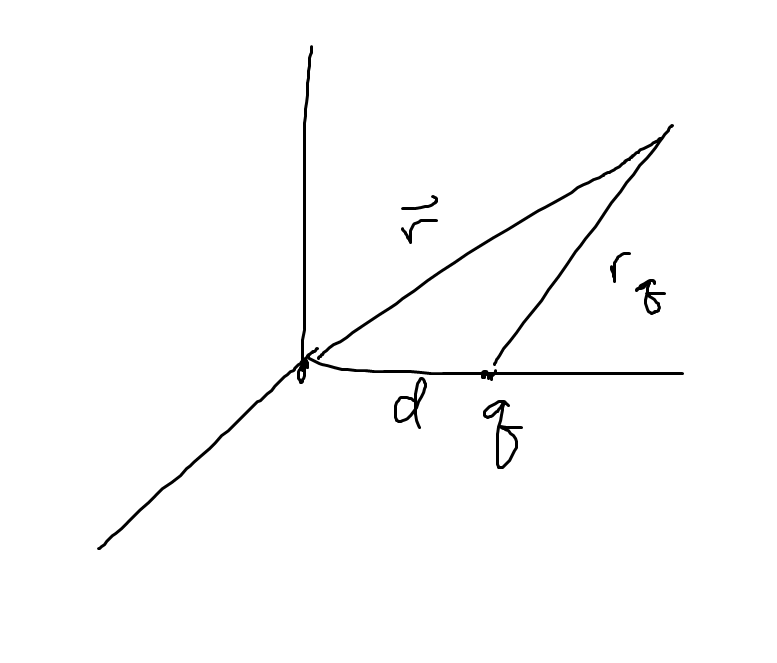
\includegraphics[width=0.4\textwidth]{Figures/08.png}
    \caption{}
    \label{fig:}
\end{figure} 
\[
    \Phi  = \frac{1}{4\pi \epsilon _0} \frac{q}{r_q}
\]
We see that this has a net dipole moment of \( \vec{p}  = q d \hat{y} \) which would have a nonzero dipole moment. Now suppose we wanted to calculate the dipole in shifted coordinates where 
\[
    \widetilde{\vec{p} } = \int  \widetilde{\vec{r} }^{\prime}  \rho(\vec{r} ^{\prime} ) dV^{\prime}  = 
    \int  \left(  \vec{r} ^{\prime} - \vec{a}  \right) \rho (\vec{r} ^{\prime} ) dV^{\prime}   
\]
\[
    = \int  \vec{r} ^{\prime} \rho (\vec{r} ^{\prime} ) dV^{\prime}  - \vec{a} \int  \rho(\vec{r} ^{\prime} ) dV^{\prime} 
\]
\[
    = \vec{p}  - \vec{a}  Q
\]
Thus, we ask where the origin is based on the dipole. 
\section{Electric field of Dipole}
\[
    \Phi_{dip} = \frac{\hat{r} \cdot \vec{p} }{4\pi \epsilon _0 r^{2} } = \frac{p \cos \theta}{4 \pi  \epsilon _0 r^{2} }
\]
where the dipole is aligned with the z-axis. We have 
\[
    E_r = - \frac{\partial \Phi_{dip} }{\partial r}, \quad E_\theta = -\frac{1}{r} \frac{\partial \Phi_{dip} }{\partial \theta}, \quad E_{\phi } = -\frac{1}{r\sin \theta} \frac{\partial \Phi_{dip} }{\partial \phi } = 0    
\]
\[
    \vec{E}_{dip} = \frac{p}{4\pi \epsilon _0 r^{3} } \left(  2 \cos \theta \hat{r} + \sin \theta \hat{\theta}  \right)  
\]
If we plot this given that we have an ideal small dipole we have 
\begin{figure}[H]
    \centering
    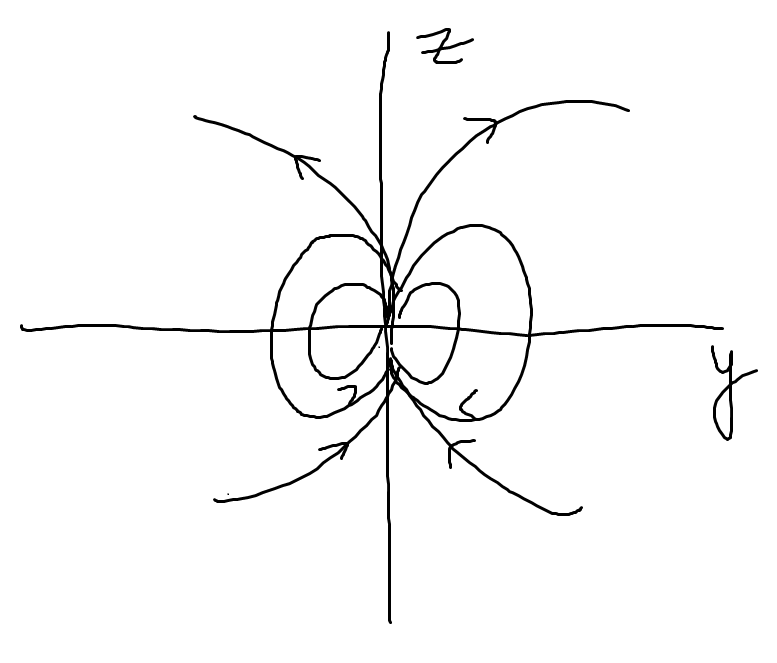
\includegraphics[width=0.4\textwidth]{Figures/09.png}
    \caption{}
    \label{fig:}
\end{figure}
If the total charge is nonzero we must find the dipole. If there is something delicate, we can use the quadrupole terms and more which tell us how the field behaves in far-field.

\chapter{Electric Fields in Matter}
\section{Polarization}
Recall that conductors have positively charged ions fixed to the lattice points while the electrons are freely moving. We can also consider dielectrics. Dielectrics are materials that don't allow current to flow. They are more often called insulators because they are the exact opposite of conductors.
\begin{figure}[H]
    \centering
    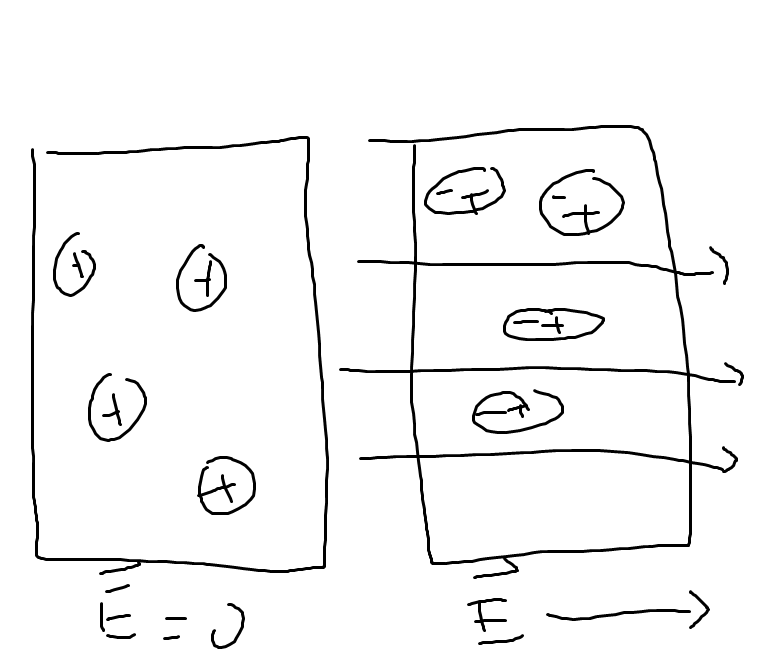
\includegraphics[width=0.5\textwidth]{Figures/10.png}
    \caption{}
    \label{fig:}
\end{figure}
This gives rise to a macroscopic polarization that we get to see. For an induced dipole which we see here we get a net dipole moment or a simplified model. 
We can show that this can be represented in the following:
\begin{figure}[H]
    \centering
    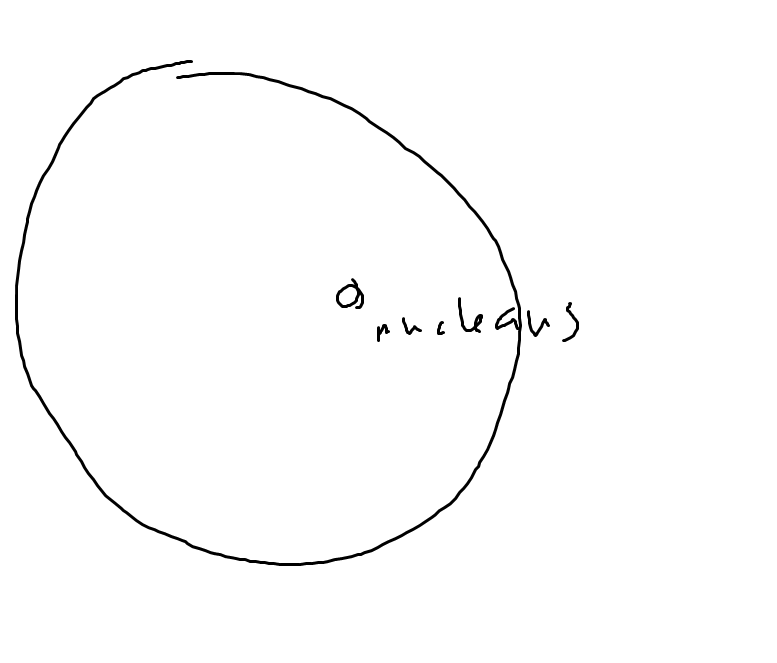
\includegraphics[width=0.4\textwidth]{Figures/11.png}
    \caption{}
    \label{fig:}
\end{figure}
When we apply a \(\vec{E} \to \) to the right, we see a shift here but we would like to know the calculation here where the shift balances the force from the external field. Thus, we can look at the force from the electron cloud to the nucleaus would be 
\[
    F_{cloud \to  nucleaus} = Ze \vec{E}_{cloud} = -Ze \vec{E}_{ext}  
\]
\[
    E_{cloud} = \frac{\rho r}{3 \epsilon _0} \hat{r} 
\]